\documentclass{article}
\usepackage{ctex}
\usepackage{amsmath}
\usepackage{tikz}
\usepackage{unicode-math}
\usetikzlibrary{arrows.meta, decorations.markings,patterns}
\begin{document}

%1.3-4 根据量子理论，氢原子中心是一个带正电 $q_e$的原子核(可以看成是点电荷),外面是带负电的电子云.在正常状态(核外电子处在s态)下，电子云的电荷密度分布是球对称的
%$$\rho_e(r)=-\frac{q_e}{\pi a_0^3}\mathrm{e}^{-\frac{2r}{a_0}}$$
%式中$a_0$ 为一常量(它相当于经典原子模型中 $s$ 电子圆形轨道的半径，称为玻尔半径)。求原子内的电场分布。

1.3-4

对半径为 $ r $ 的球面用高斯定律:

$$\oiint_S \mathbf{E} \cdot d\mathbf{S} = \frac{Q(r)}{\varepsilon_0}$$

其中 $ Q(r) $ 是半径为 $ r $ 的球内的总电荷(包括原子核和电子云)。

$$Q(r) = q_e + \int_0^r \rho_e(r') \cdot 4\pi r'^2 \, dr'$$

在半径 $ r $ 内的电荷

$$Q(r) = q_e+\int_0^r \left[ -\frac{q_e}{\pi a_0^3} e^{\frac{2r'}{a_0}} \right] \cdot 4\pi r'^2 \, dr'= q_e-\frac{4q_e}{a_0^3} \int_0^r r'^2 e^{\frac{2r'}{a_0}} \, dr'$$

令
$$ x = \frac{2r'}{a_0} , r' = \frac{a_0}{2} x , dr' = \frac{a_0}{2} dx $$

$$\int_0^r r'^2 e^{\frac{2r'}{a_0}} dr' = \frac{a_0^3}{8} \int_0^{\frac{2r}{a_0}} x^2 e^{-x} dx$$

$$Q(r)= \frac{q_e}{2} e^{-\frac{2r}{a_0}}((\frac{2r}{a_0})^2 + 2\frac{2r}{a_0} + 2)$$

高斯定律:
$$E(r) \cdot 4\pi r^2 = \frac{Q(r)}{\varepsilon_0}$$
$$E(r) = \frac{Q(r)}{4\pi \varepsilon_0 r^2}= \frac{q_e}{8\pi \varepsilon_0 r^2} \, e^{-\frac{2r}{a_0}} \left[ \left( \frac{2r}{a_0} \right)^2 + 2\left( \frac{2r}{a_0} \right) + 2 \right]$$

所以:
$$E(r) = \frac{q_e}{4\pi \varepsilon_0 r^2} \, e^{-\frac{2r}{a_0}} \left( \frac{2r^2}{a_0^2} + \frac{2r}{a_0} + 1 \right)$$

原子内的电场分布(球对称，径向)为:

$$E(r) = \frac{q_e}{4\pi\varepsilon_0 r^2} \, e^{-\frac{2r}{a_0}} \left[ 1 + \frac{2r}{a_0} + \frac{2r^2}{a_0^2} \right]$$

方向沿径向(若 $ q_e > 0 $，则 $ E(r) > 0 $，向外)




\newpage

%1.3-7 一对无限长的共轴直圆简，半径分别为$R_1$和$R_2$,筒面上都均匀带电.沿轴线单位长度的电荷量分别为$\lambda_1$ 和 $\lambda _2$. 求各区域内的场强分布;
%若 $\lambda_1=-\lambda_2$,情况如何？画出此情形的 $E-r$ 曲线.

1.3-7

由于轴对称性，电场方向沿径向，大小只与到轴的距离 $ r $ 有关。
  
用高斯定理:取高为 $ h $、半径为 $ r $ 的同轴圆柱面作为高斯面。

对于无限长圆柱面，由高斯定理:
$$\oiint_S \mathbf{E} \cdot d\mathbf{S} = \frac{Q}{\varepsilon_0}$$

其中 $ Q $ 是高斯面内包围的电荷(单位长度电荷量乘以高 $ h $)。

圆柱侧面积 $ 2\pi r h $，电场垂直于侧面且大小恒定，所以:
$$E(r) \cdot 2\pi r h = \frac{Q}{\varepsilon_0}$$
$$E(r) = \frac{Q / h}{2\pi \varepsilon_0 r}$$

记 $ \lambda = Q / h $ 为高斯面内单位长度的电荷量。


 (1) 区域 I:$ 0 < r < R_1 $
高斯面内无电荷(因为电荷都在圆柱面上):
$$\lambda = 0 \quad \Rightarrow \quad E(r) = 0$$

 (2) 区域 II:$ R_1 < r < R_2 $
高斯面含内圆柱面电荷，但不含外圆柱面电荷:
$$\lambda = \lambda_1\quad \Rightarrow E(r) = \frac{\lambda_1}{2\pi \varepsilon_0 r}$$


 (3) 区域 III:$ r > R_2 $
高斯面包含两个圆柱面的电荷:
$$\lambda = \lambda_1 + \lambda_2\quad \Rightarrow E(r) = \frac{\lambda_1 + \lambda_2}{2\pi \varepsilon_0 r}$$


$$E(r) =
\begin{cases}
0, & 0 < r < R_1 \\[4pt]
\displaystyle \frac{\lambda_1}{2\pi \varepsilon_0 r}, & R_1 < r < R_2 \\[8pt]
\displaystyle \frac{\lambda_1 + \lambda_2}{2\pi \varepsilon_0 r}, & r > R_2
\end{cases}$$


\newpage
特殊情况 $\lambda_1 = -\lambda_2$

设 $\lambda_1 = \lambda$，$\lambda_2 = -\lambda$。

 区域 I:$ r < R_1 $
$$E = 0$$

 区域 II:$ R_1 < r < R_2 $
$$E = \frac{\lambda}{2\pi \varepsilon_0 r}$$

 区域 III:$ r > R_2 $
$$\lambda = \lambda + (-\lambda) = 0$$
$$E = 0$$

所以:
$$
E(r) =
\begin{cases}
0, & 0 < r < R_1 \\[4pt]
\displaystyle \frac{\lambda}{2\pi \varepsilon_0 r}, & R_1 < r < R_2 \\[8pt]
0, & r > R_2
\end{cases}
$$





\begin{tikzpicture}[>=Stealth, scale=1.5]
    % 定义参数
    \def\Rone{2}
    \def\Rtwo{4}
    \def\Emax{2.5}   % E 的最大值(在 r=R1 处)
    
    % 坐标轴
    \draw[->] (0,0) -- (6,0) node[right] {$r$};
    \draw[->] (0,-0.5) -- (0,3) node[above] {$E(r)$};
    
    % 标注 R1, R2
    \draw[dashed] (\Rone,0) -- (\Rone, \Emax);
    \draw[dashed] (\Rtwo,0) -- (\Rtwo, 0.8*\Emax);
    \node[below] at (\Rone,0) {$R_1$};
    \node[below] at (\Rtwo,0) {$R_2$};
    
    % 计算 E 在 R1 和 R2 的值(按 1/r 规律)
    \pgfmathsetmacro{\EatRone}{\Emax}
    \pgfmathsetmacro{\EatRtwo}{\Emax*\Rone/\Rtwo}
    
    % 画 E(r) 曲线
    \draw[very thick, blue] (0,0) -- (\Rone,0);  % 区域 I: r < R1
    \draw[thick,blue,domain=2:4,samples=100] plot (\x,{5/\x});
    \draw[very thick, blue] (\Rtwo,0) -- (6,0);  % 区域 III: r > R2
    
    % 在 R1 处画跳跃(用空心圆和实心圆表示间断点)
    \draw[fill=white] (\Rone,0) circle (2pt);
    \draw[fill=blue] (\Rone,\EatRone) circle (2pt);
    
    % 在 R2 处画跳跃
    \draw[fill=blue] (\Rtwo,\EatRtwo) circle (2pt);
    \draw[fill=white] (\Rtwo,0) circle (2pt);
    
    % 标注公式
    \node[above right, blue] at (2.8, 1.8) {$E(r) = \dfrac{\lambda_1}{2\pi\varepsilon_0 r}$};
    \node at (1, -0.3) {$E=0$};
    \node at (5, -0.3) {$E=0$};
    
    % 标题
    \node[above] at (3, 3) {$\lambda_1 = -\lambda_2$ 时的 $E$-$r$ 曲线};
\end{tikzpicture}









\newpage

%1.3-12 三个无限大的平行平面都均匀带电，电荷面密度分别为 $\sigma_{e1}$、$\sigma_{e2}$、$\sigma_{e3}$．求下列情况各处的场强:

%(1)$\sigma_{e1} = \sigma_{e2} = \sigma_{e3} = \sigma_e$;

%(2)$\sigma_{e1} = \sigma_{e3} = \sigma_e$，$\sigma_{e2} = -\sigma_e$;

%(3)$\sigma_{e1} = \sigma_{e3} = -\sigma_e$，$\sigma_{e2} = \sigma_e$;

%(4)$\sigma_{e1} = \sigma_e$，$\sigma_{e2} = \sigma_{e3} = -\sigma_e$．

1.3-12

设平面 1 在 $x=0$，平面 2  $x=d$，平面 3  $x=2d$($d>0$)

则空间被分成 4 个区域:

区域 I:$x < 0$(平面 1 左侧)

区域 II:$0 < x < d$(平面 1 与平面 2 之间)

区域 III:$d < x < 2d$(平面 2 与平面 3 之间)

区域 IV:$x > 2d$(平面 3 右侧)

各平面单独场强大小均为 $E_0 = \frac{\sigma_e}{2\varepsilon_0}$。

(1) $\sigma_1 = \sigma_2 = \sigma_3 = \sigma_e$

区域 I:
平面 1:$-E_0$;
平面 2:$-E_0$;
平面 3:$-E_0$;
$E_I =-3E_0 = -\frac{3\sigma_e}{2\varepsilon_0}$

区域 II:
平面 1:$+E_0$;
平面 2:$-E_0$;
平面 3:$-E_0$;
$E_{II} =-E_0 = -\frac{\sigma_e}{2\varepsilon_0}$

区域 III:
平面 1:$+E_0$;
平面 2:$+E_0$;
平面 3:$-E_0$;
$E_{III} =E_0 = \frac{\sigma_e}{2\varepsilon_0}$

区域 IV:
平面 1:$+E_0$;
平面 2:$+E_0$;
平面 3:$+E_0$;
$E_{IV}= 3E_0 = \frac{3\sigma_e}{2\varepsilon_0}$

$$E =
\begin{cases}
-\dfrac{3\sigma_e}{2\varepsilon_0}, & x<0 \\[6pt]
-\dfrac{\sigma_e}{2\varepsilon_0}, & 0<x<d \\[6pt]
\dfrac{\sigma_e}{2\varepsilon_0}, & d<x<2d \\[6pt]
\dfrac{3\sigma_e}{2\varepsilon_0}, & x>2d
\end{cases}
$$
 
 (2) $\sigma_1 = \sigma_3 = \sigma_e,\sigma_2 = -\sigma_e$

区域 I:
平面 1 :$-E_0$;
平面 2 :$+E_0$;
平面 3 :$-E_0$;
$E_I =-E_0 = -\frac{\sigma_e}{2\varepsilon_0}$

 区域 II:
平面 1:$+E_0$;
平面 2 :$+E_0$;
平面 3:$-E_0$;
$E_{II} =E_0 = \frac{\sigma_e}{2\varepsilon_0}$

 区域 III:
平面 1:$+E_0$;
平面 2:$-E_0$;
平面 3:$-E_0$;
$E_{III} =-E_0 = -\frac{\sigma_e}{2\varepsilon_0}$

 区域 IV:
平面 1:$+E_0$;
平面 2:$-E_0$;
平面 3:$+E_0$;
$E_{IV} = E_0 = \frac{\sigma_e}{2\varepsilon_0}$
$$
E =
\begin{cases}
-\dfrac{\sigma_e}{2\varepsilon_0}, & x<0 \\[6pt]
\dfrac{\sigma_e}{2\varepsilon_0}, & 0<x<d \\[6pt]
-\dfrac{\sigma_e}{2\varepsilon_0}, & d<x<2d \\[6pt]
\dfrac{\sigma_e}{2\varepsilon_0}, & x>2d
\end{cases}
$$

\newpage

(3)  $\sigma_1 = \sigma_3 = -\sigma_e,\sigma_2 = \sigma_e$

区域 I:
平面 1:$+E_0$;
平面 2:$-E_0$;
平面 3:$+E_0$;
$E_I =E_0 = \frac{\sigma_e}{2\varepsilon_0}$

区域 II:
平面 1:$-E_0$;
平面 2:$-E_0$;
平面 3:$+E_0$;
$E_{II} =-E_0 = -\frac{\sigma_e}{2\varepsilon_0}$

区域 III:
平面 1:$-E_0$;
平面 2:$+E_0$;
平面 3:$+E_0$;
$E_{III} =E_0 = \frac{\sigma_e}{2\varepsilon_0}$

区域 IV:
平面 1:$-E_0$;
平面 2:$+E_0$;
平面 3:$-E_0$;
$E_{IV}= -E_0 = -\frac{\sigma_e}{2\varepsilon_0}$

$$E =
\begin{cases}
\dfrac{\sigma_e}{2\varepsilon_0}, & x<0 \\[6pt]
-\dfrac{\sigma_e}{2\varepsilon_0}, & 0<x<d \\[6pt]
\dfrac{\sigma_e}{2\varepsilon_0}, & d<x<2d \\[6pt]
-\dfrac{\sigma_e}{2\varepsilon_0}, & x>2d
\end{cases}
$$
 
 (4) $\sigma_1 = \sigma_e,\sigma_2 = \sigma_3 = -\sigma_e$

区域 I:
平面 1 :$-E_0$;
平面 2 :$+E_0$;
平面 3 :$+E_0$;
$E_I =E_0 = \frac{\sigma_e}{2\varepsilon_0}$

 区域 II:
平面 1:$+E_0$;
平面 2 :$+E_0$;
平面 3:$+E_0$;
$E_{II} =3E_0 = \frac{3\sigma_e}{2\varepsilon_0}$

 区域 III:
平面 1:$+E_0$;
平面 2:$-E_0$;
平面 3:$+E_0$;
$E_{III} =E_0 = \frac{\sigma_e}{2\varepsilon_0}$

 区域 IV:
平面 1:$+E_0$;
平面 2:$-E_0$;
平面 3:$-E_0$;
$E_{IV} = -E_0 = -\frac{\sigma_e}{2\varepsilon_0}$
$$
E =
\begin{cases}
\dfrac{\sigma_e}{2\varepsilon_0}, & x<0 \\[6pt]
\dfrac{3\sigma_e}{2\varepsilon_0}, & 0<x<d \\[6pt]
\dfrac{\sigma_e}{2\varepsilon_0}, & d<x<2d \\[6pt]
-\dfrac{\sigma_e}{2\varepsilon_0}, & x>2d
\end{cases}
$$

\begin{table}[ht]
\centering
\begin{tabular}{|c|c|c|c|c|}
\hline
情况 & 区域 I & 区域 II & 区域 III & 区域 IV \\
\hline
(1) $\sigma_1=\sigma_2=\sigma_3=\sigma_e$ & $-\frac{3\sigma_e}{2\varepsilon_0}$ & $-\frac{\sigma_e}{2\varepsilon_0}$ & $\frac{\sigma_e}{2\varepsilon_0}$ & $\frac{3\sigma_e}{2\varepsilon_0}$ \\
\hline
(2) $\sigma_1=\sigma_3=\sigma_e,\ \sigma_2=-\sigma_e$ & $-\frac{\sigma_e}{2\varepsilon_0}$ & $\frac{\sigma_e}{2\varepsilon_0}$ & $-\frac{\sigma_e}{2\varepsilon_0}$ & $\frac{\sigma_e}{2\varepsilon_0}$ \\
\hline
(3) $\sigma_1=\sigma_3=-\sigma_e,\ \sigma_2=\sigma_e$ & $\frac{\sigma_e}{2\varepsilon_0}$ & $-\frac{\sigma_e}{2\varepsilon_0}$ & $\frac{\sigma_e}{2\varepsilon_0}$ & $-\frac{\sigma_e}{2\varepsilon_0}$ \\
\hline
(4) $\sigma_1=\sigma_e,\ \sigma_2=\sigma_3=-\sigma_e$ & $\frac{\sigma_e}{2\varepsilon_0}$ & $\frac{3\sigma_e}{2\varepsilon_0}$ & $\frac{\sigma_e}{2\varepsilon_0}$ & $-\frac{\sigma_e}{2\varepsilon_0}$ \\
\hline
\end{tabular}
\end{table}



\newpage

%1.3-14 在半导体 pn 结附近总是堆积着正、负电荷,在 n 区内有正电荷, p 区内有负电荷,两区电荷的代数和为零. 
%我们把 pn 结看成是一对带正、负电荷的无限大平板,它们相互接触. 取坐标 $x$ 的原点在 p、n区的交界面上, 
%n 区的范围是 $-x_n \leq x \leq 0$, p 区的范围是 $0 \leq x \leq x_p$ . 设两区内电荷体分布都是均匀的
%$$\begin{cases}\text{n 区}:\rho_\mathrm{e}(x)=N_\mathrm{p}e\\\\\text{p 区}:\rho_\mathrm{e}(x)=-N_\mathrm{A}e\end{cases}$$
%这里 $N_D,N_A$是常量,且$N_Ax_p=N_Dx_n$(两区电荷数量相等).试证明电场的分布为

%$$\begin{cases}\text{n 区:}&E(x)=\frac{N_\mathrm{D}e}{\varepsilon_0}(x_\mathrm{n}+x)\\\\\text{p 区:}&E(x)=\frac{N_\mathrm{A}e}{\varepsilon_0}(x_\mathrm{p}-x)\end{cases}$$

1.3-14

\begin{minipage}[b]{0.5\linewidth}
电荷分布：
$$
\rho_e(x) =
\begin{cases}
N_D e, & -x_n \le x \le 0  \\
-N_A e, & 0 \le x \le x_p  
\end{cases}
$$
其中 $N_D, N_A, e > 0$，且满足：
$$N_A x_p = N_D x_n$$
$$Q_{\text{总}}= N_D x_n\cdot S-N_A x_p\cdot S =0$$
\vspace{0.5em}
\end{minipage}
\hfill
\begin{minipage}[b]{0.4\linewidth}
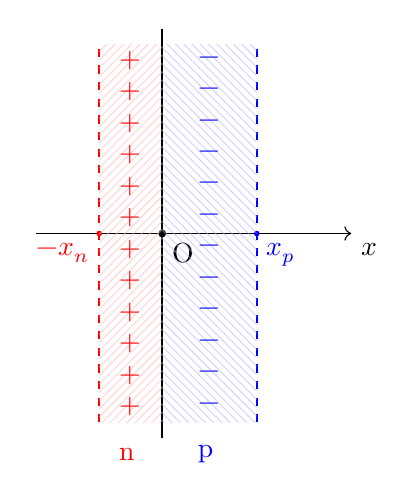
\begin{tikzpicture}[scale=0.4]
    % 坐标系
    \draw[->] (-4,0) -- (6,0); % x轴
    \draw[thick] (0,-6.5) -- (0,6.5); % y轴（加粗，不标箭头）
    
    % 垂直线 x = x_p = 3
    \draw[dashed, blue, thick] (3,-6) -- (3,6);
    % 垂直线 x = -x_n = -2
    \draw[dashed, red, thick] (-2,-6) -- (-2,6);
    
    % 标注点
    \filldraw[blue] (3,0) circle (2pt) node[below right] {$x_p$};
    \filldraw[black] (0,0) circle (3pt) node[below right] {$\rm{O}$};
    \filldraw[red] (-2,0) circle (2pt) node[below left] {$-x_n$};
    
    % 区域填充和标注
    % n区：x=-2 与 y轴之间
    \fill[pattern=north east lines, pattern color=red!30, opacity=0.5] 
        (-2,-6) rectangle (0,6);
    \node[red] at (-1, -7) {n区};
    
    % p区：x=3 与 y轴之间
    \fill[pattern=north west lines, pattern color=blue!30, opacity=0.5] 
        (0,-6) rectangle (3,6);
    \node[blue] at (1.5, -7) {p区};

    
    % 坐标轴标签
    \node[below right] at (6,0) {$x$};
    
    % 添加+号和-号
    \foreach \y in {-5.5,-4.5,...,5.5}
    {
        % n区：+号
        \node[red] at (-1, \y) {$+$};
        % p区：-号
        \node[blue] at (1.5, \y) {$-$};
    }
\end{tikzpicture}
\end{minipage}


取高斯面为底面积为 $S$ 的柱面，柱面两个底面的分别在 $x$ 和0

由对称性，电场只有 $x$ 分量 $E(x)$，且只与 $x$有关

设柱面内总电量为Q
$$Q=\int_{0}^{x} \rho_e(x)Sdx\Rightarrow \frac{Q}{S}=\int_{0}^{x}\rho_e(x)dx$$

高斯定律：

$$\oiint_S \mathbf{E} \cdot d\mathbf{S} = \frac{Q}{\varepsilon_0}$$

考虑到S与E垂直

$$\oiint_S \mathbf{E} \cdot d\mathbf{S}=E(x)S+E(0)S=\frac{Q}{S\varepsilon_0}=\frac{\int_{0}^{x}\rho_e(x)dx}{\varepsilon_0}$$

对x求导有

$$\frac{dE}{dx}=\frac{\rho_e(x)}{\varepsilon_0}$$

\vspace{1em}
\begin{minipage}[b]{0.4\linewidth}
(1) 在 n 区 ($-x_n \le x \le 0$)
$$\frac{dE}{dx} = \frac{N_D e}{\varepsilon_0}$$
积分：
$$E(x) = \frac{N_D e}{\varepsilon_0} x + E(0^-)$$
\end{minipage}
\hfill
\begin{minipage}[b]{0.5\linewidth}
(2) 在 p 区 ($0 \le x \le x_p$)

$$\frac{dE}{dx} = -\frac{N_A e}{\varepsilon_0}$$
积分：
$$E(x) = -\frac{N_A e}{\varepsilon_0} x + E(0^+)$$
\end{minipage}

\newpage

在 $x = 0$ 处，电场连续：
$$E(0^-) = E(0^+)=E(0)\qquad\frac{N_D e}{\varepsilon_0} \cdot 0 + E(0^-) = -\frac{N_A e}{\varepsilon_0} \cdot 0 + E(0^+)$$

在 $x = -x_n$ 处，左侧无电荷，电场为零：$E(-x_n) = 0$

代入 n 区公式：

$$\frac{N_D e}{\varepsilon_0} (-x_n) + E(0) = 0$$
$$E(0)= \frac{N_D e}{\varepsilon_0} x_n$$
由于
$$N_A x_p = N_D x_n$$
有
$$E(0)= \frac{N_A e}{\varepsilon_0} x_p$$

代入可得

$$\begin{cases}\text{n 区:}&E(x)=\frac{N_\mathrm{D}e}{\varepsilon_0}(x_\mathrm{n}+x)\\\\\text{p 区:}&E(x)=\frac{N_\mathrm{A}e}{\varepsilon_0}(x_\mathrm{p}-x)\end{cases}$$



\begin{minipage}[b]{0.43\linewidth}
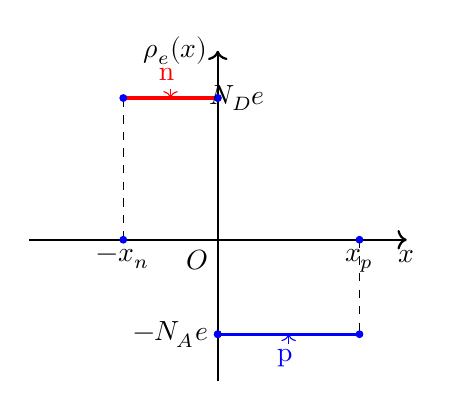
\begin{tikzpicture}[scale=0.6]
    % 坐标系
    \draw[->, thick] (-4,0) -- (4,0) node[below] {$x$};
    \draw[->, thick] (0,-3) -- (0,4) node[left] {$\rho_e(x)$};
    
    % 原点标注
    \node[below left] at (0,0) {$O$};
    
    % 关键点标注
    \draw[dashed] (-2,0) -- (-2,3);
    \draw[dashed] (3,0) -- (3,-2);
    \draw[dashed] (0,3) -- (-2,3);
    \draw[dashed] (0,-2) -- (3,-2);
    
    % 绘制分段函数
    \draw[very thick, red] (-2,3) -- (0,3);   % 第一段：-2 ≤ x ≤ 0
    \draw[very thick, blue] (0,-2) -- (3,-2);  % 第二段：0 ≤ x ≤ 3
    
    % 空心点（不连续点）
    \draw[fill=white] (0,3) circle (2pt);
    \draw[fill=white] (0,-2) circle (2pt);
    
    % 实心点（端点）
    \filldraw[blue] (-2,3) circle (2pt);
    \filldraw[blue] (3,-2) circle (2pt);
    \filldraw[blue] (-2,0) circle (2pt);
    \filldraw[blue] (0,3) circle (2pt);
    \filldraw[blue] (0,-2) circle (2pt);
    \filldraw[blue] (3,0) circle (2pt);
    
    % 特殊点标注
    \node[below] at (-2,0) {$-x_n$};
    \node[below] at (3,0) {$x_p$};
    \node[left] at (1.2,3) {$N_De$};
    \node[left] at (0,-2) {$-N_Ae$};
    
    % 添加区域标注
    \node[red] at (-1, 3.5) {n区};
    \node[blue] at (1.5, -2.5) {p区};
    
    % 添加箭头说明
    \draw[->, red] (-1, 3.2) -- (-1, 3);
    \draw[->, blue] (1.5, -2.2) -- (1.5, -2);
\end{tikzpicture}
\end{minipage}
\hfill
\begin{minipage}[b]{0.5\linewidth}
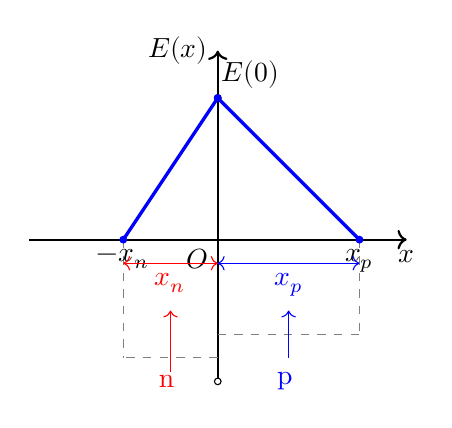
\begin{tikzpicture}[scale=0.6]
    % 坐标系
    \draw[->, thick] (-4,0) -- (4,0) node[below] {$x$};
    \draw[->, thick] (0,-3) -- (0,4) node[left] {$E(x)$};
    
    % 原点标注
    \node[below left] at (0,0) {$O$};
    
    % 关键点标注
    \draw[dashed, gray] (-2,0) -- (-2,-2.5);
    \draw[dashed, gray] (3,0) -- (3,-2);
    \draw[dashed, gray] (0,-2.5) -- (-2,-2.5);
    \draw[dashed, gray] (0,-2) -- (3,-2);
    
    % 计算关键点
    % 当 x = -2 时：E(-2) = 3(-2+2) = 0
    % 当 x = 0 时：E(0) = 3(0+2) = 6
    % 当 x = 0 时：E(0) = -2(3-0) = -6（另一段）
    % 当 x = 3 时：E(3) = -2(3-3) = 0
    
    % 绘制分段函数
    \draw[very thick, blue] (-2,0) -- (0,3);   % 第一段：-2 ≤ x ≤ 0
    \draw[very thick, blue] (0,3) -- (3,0);   % 第二段：0 ≤ x ≤ 3
    
    % 空心点（不连续点）
    \draw[fill=white] (0,3) circle (2pt);
    \draw[fill=white] (0,-3) circle (2pt);
    
    % 实心点（端点）
    \filldraw[blue] (-2,0) circle (2pt);
    \filldraw[blue] (0,3) circle (2pt);
    \filldraw[blue] (3,0) circle (2pt);
    

    
    % 特殊点标注
    \node[below] at (-2,0) {$-x_n$};
    \node[below] at (3,0) {$x_p$};
    \node[left] at (1.5,3.5) {$E(0)$};
    
    % 添加区域标注
    \node[red] at (-1, -3) {n区};
    \node[blue] at (1.5, -3) {p区};
    
    % 添加箭头说明
    \draw[->, red] (-1, -2.8) -- (-1, -1.5);
    \draw[->, blue] (1.5, -2.5) -- (1.5, -1.5);
    
    
    % 添加最大值标注
    \draw[<->, red] (-2,-0.5) -- (0,-0.5) node[midway, below] {$x_n$};
    \draw[<->, blue] (0,-0.5) -- (3,-0.5) node[midway, below] {$x_p$};
\end{tikzpicture}
\end{minipage}













\newpage

%2.有一高斯面$S$,$S$内有一点电荷$Q_1$,$S$外有一点电荷$Q_2$,$S$面上有一点电荷$Q_3$，求$S$的电通量。

2

高斯定理
$$\Phi_E = \oiint_S \mathbf{E} \cdot d\mathbf{S} = \frac{Q}{\varepsilon_0}$$  

其中 $ Q $ 是 高斯面内部 的电荷。  

$ Q_1 $ 在 $ S $ 内;
$ Q_2 $ 在 $ S $ 外 ;
$ Q_3 $ 在 $ S $ 面上 

所以：
  
$$Q = Q_1$$

$$\Phi_E = \frac{Q_1}{\varepsilon_0}$$  





\newpage

3

通过一个任意闭合曲面 S 的电场强度通量 $\Phi_\mathrm{E}$等于该面所包围的所有电荷量的代数和$\Sigma q$ 除以$\boldsymbol{\varepsilon}_0$,与闭合面外的电荷无关.
用公式来表达高斯定理，则有

$$\Phi_E=\oiint_SE\cos\theta\mathrm{d}S=\frac1{\varepsilon_0}\sum_{(S\text{内})}q_i$$

这里$\oiint _S$表 示 沿 一 个 闭 合 曲 面  S 的 积 分 , 这 闭 合 曲 面  $S$ 习惯上叫作高斯面.

\end{document}